%%%%%%%%%%%%%%%%%%%%%%%%%%%%%%%%%%%%%%%%%%%%%%%%%%%%%%%%%%%%%%%%%%%%%%%%%%%%%%%%
%%%%%%%%%%%%%%%%%%%%%%%%%%%%%%%%%%%%%%%%%%%%%%%%%%%%%%%%%%%%%%%%%%%%%%%%%%%%%%%%
%
% A general frame for lecture slides and lecture notes in one file
% using LaTeX beamer
%
%%%%%%%%%%%%%%%%%%%%%%%%%%%%%%%%%%%%%%%%%%%%%%%%%%%%%%%%%%%%%%%%%%%%%%%%%%%%%%%%
%%%%%%%%%%%%%%%%%%%%%%%%%%%%%%%%%%%%%%%%%%%%%%%%%%%%%%%%%%%%%%%%%%%%%%%%%%%%%%%%

% only for the article version
\mode<article>
{
  \usepackage[automark,komastyle]{scrpage2}
  \usepackage{amsfonts}
  \usepackage{amscd}
  %\usepackage[headings]{fullpage}
%  \setlength{\parindent}{0pt}
%  \setlength{\parskip}{1.25ex plus 0.5ex minus 0.2ex}
}

% only presentation
\mode<presentation>
{
%  \usepackage{times}
%  \usetheme{default}
  \usepackage{multimedia}
  \usetheme[secheader]{Boadilla}
  \setbeamercovered{transparent}
  \setbeamertemplate{background canvas}[vertical shading][bottom=white!10,top=white!10]
  \setlength{\parindent}{0pt}
  \setlength{\parskip}{1.35ex plus 0.5ex minus 0.3ex}
  \setbeamertemplate{theorems}[numbered]
  \usefonttheme[onlysmall]{structurebold}
  \usepackage{amscd}
}

%% support '.' in pdf file names
\usepackage{grffile}

% all after
\usepackage{tikz}
\usepackage{eurosym}
\usepackage{graphicx}
%\usepackage{psfrag}
\usepackage{listings}
\lstset{language=C++, basicstyle=\ttfamily,
  keywordstyle=\color{red}\bfseries, tabsize=4, stringstyle=\ttfamily,
  commentstyle=\itshape, extendedchars=true, inputencoding=utf8, texcl=true, escapeinside={/*@}{@*/}}
\usepackage{curves}
%\usepackage{epic}
\usepackage{calc}
\usepackage{picinpar}
%\usepackage{fancybox}
%\usepackage{xspace}
\usepackage{enumerate}
\usepackage{algorithmic}
\usepackage{algorithm}
\usepackage{bm}
\usepackage[german]{varioref}
\usepackage{bibgerm}
%\usepackage{multibib}
\usepackage{nicefrac}
\usepackage{cite}

\mode<article> {
%  \usepackage[dvips,a4paper]{hyperref}
  \usepackage[%
  pagebackref=false, % bibliography -> text
  linktocpage=true, % toc etc: make page number active (not name)
  plainpages=false, % distinguish roman and arabic pagenumbers
  bookmarksopen=true,%
  bookmarksnumbered=true,%
  pdfauthor={Peter Bastian},%
  pdftitle={Heidelberger Numerikbibliothek für die Lehre},%
  pdfsubject={},%
  pdfkeywords={},%
]{hyperref}        % clickabe references
  \usepackage{multimedia}
  \usepackage{cite}
  \setkomafont{pagenumber}{\normalfont\scshape}
  \setkomafont{pageheadfoot}{\normalfont\scshape}
}
%\usepackage{breakurl}

%\newcites{num}{Lehrbücher Numerik}
%\newcites{cpp}{Lehrbücher C++}

%The theorems
\mode<presentation>
{
\theoremstyle{definition}
}
\mode<article>
{
\theoremstyle{definition}
}

\newtheorem{Def}{Definition}[section]
\newtheorem{Bsp}[Def]{Beispiel}
\newtheorem{Bem}[Def]{Bemerkung}
\newtheorem{Lem}[Def]{Lemma}
\newtheorem{Rgl}[Def]{Regel}
\newtheorem{Sat}[Def]{Satz}
\newtheorem{HSatz}[Def]{Hilfssatz}
\newtheorem{Kor}[Def]{Korollar}
\newtheorem{Folg}[Def]{Folgerung}
\newtheorem{Beob}[Def]{Beobachtung}
\newtheorem{wissen}[Def]{Wissen}
\newtheorem*{geschichte}{Geschichte}


%\newtheorem{Def}{Definition}[section]
%\newtheorem{Exm}[Def]{Example}
%\newtheorem{Lem}[Def]{Lemma}
%\newtheorem{Rem}[Def]{Remark}
%\newtheorem{Rul}[Def]{Rule}
%\newtheorem{Thm}[Def]{Theorem}
%\newtheorem{Cor}[Def]{Corollary}
%\newtheorem{Obs}[Def]{Observation}
%\newtheorem{Ass}[Def]{Assumption}
%\newtheorem{Pro}[Def]{Property}
%\newtheorem{Alg}[Def]{Algorithm}
%\newtheorem{Prp}[Def]{Proposition}
%\newtheorem{Lst}[Def]{Listing}

% Delete this, if you do not want the table of contents to pop up at
% the beginning of each subsection:
%\AtBeginSection[]
%{
%  \begin{frame}<beamer>
%    \frametitle{Contents}
%\tableofcontents[currentsection,sectionstyle=show/hide,subsectionstyle=show/show/hide]
%    \tableofcontents[currentsection]
%  \end{frame}
%}

% Title definition
\mode<presentation>
{
  \title[HDNum]{Heidelberger Numerikbibliothek für die Lehre}
  \author{Peter Bastian}
  \institute[IWR]
  {
    Universität Heidelberg\\
    Interdisziplinäres Zentrum für Wissenschaftliches Rechnen\\
    Im Neuenheimer Feld 205, D-69120 Heidelberg\\
	email: \url{Peter.Bastian@iwr.uni-heidelberg.de}
  }
  \date{\today}
  \logo{\includegraphics[width=9mm]{./EPS/iwrlogo-klein}}
}
\mode<article>
{
  \title{Heidelberger Numerikbibliothek \\ für die Lehre}
  \author{\textsc{Peter Bastian}\\
    Universität Heidelberg\\
    Interdisziplinäres Zentrum für Wissenschaftliches Rechnen\\
    Im Neuenheimer Feld 205, D-69120 Heidelberg\\
	email: \url{Peter.Bastian@iwr.uni-heidelberg.de}
  }
  \date{\today}
}

% logo nach oben
\mode<presentation>
{
% No navigation symbols and no lower logo
\setbeamertemplate{sidebar right}{}

% logo
\newsavebox{\logobox}
\sbox{\logobox}{%
    \hskip\paperwidth%
    \rlap{%
      % putting the logo should not change the vertical possition
      \vbox to 0pt{%
        \vskip-\paperheight%
        \vskip0.35cm%
        \llap{\insertlogo\hskip0.1cm}%
        % avoid overfull \vbox messages
        \vss%
      }%
    }%
}

\addtobeamertemplate{footline}{}{%
    \usebox{\logobox}%
}
}

% number equations within sections in article mode
%\numberwithin{equation}{section}

% math symbols
\newcommand{\diffd}{\,d}

%%%%%%%%%%%%%%%%%%%%%%%%%%%%%%%%%%%%%%%%%%%%%%%%%%%%%%%%%%%%%%%%%%%%%%%%%%%%%%%%
%%%%%%%%%%%%%%%%%%%%%%%%%%%%%%%%%%%%%%%%%%%%%%%%%%%%%%%%%%%%%%%%%%%%%%%%%%%%%%%%
%
% now comes the individual stuff lecture by lecture
%
%%%%%%%%%%%%%%%%%%%%%%%%%%%%%%%%%%%%%%%%%%%%%%%%%%%%%%%%%%%%%%%%%%%%%%%%%%%%%%%%
%%%%%%%%%%%%%%%%%%%%%%%%%%%%%%%%%%%%%%%%%%%%%%%%%%%%%%%%%%%%%%%%%%%%%%%%%%%%%%%%
\mode<article>
{
\pagestyle{scrheadings}
}

\begin{document}
\nocite{*}
\mode<presentation>
{
  \begin{frame}
    \titlepage
  \end{frame}
}
\mode<article>
{
\maketitle
}

\begin{abstract}
Die Heidelberger Numerikbibliothek wurde begleitend zu den Vorlesungen
\textit{Einführung in die Numerik} und \textit{Numerik} in der Programmiersprache C++
entwickelt und stellt
einfach zu benutzende Klassen für grundlegende Aufgaben in der Numerik bis hin zur Lösung
von gewöhnlichen Differentialgleichungen zur Verfügung. In fast allen Klassen ist der
benutzte Zahlentyp parametrisierbar so dass auch hochpräzise Rechnungen durchgeführt werden können.
\end{abstract}

%\mode<presentation>{
%\begin{frame}<presentation>
%\frametitle{Outline}
%\tableofcontents[section,sectionstyle=show/show,subsectionstyle=hide/hide/hide]
%\end{frame}
%}

\mode<article>
{
\tableofcontents
}

\mode<all>{
}


%%%%%%%%%%%%%%%%%%%%%%%%%%%%%%%%%%%%%%%%%%%%%%%%%%%%%%%%%%%%%%%
% Die Kapitel
%%%%%%%%%%%%%%%%%%%%%%%%%%%%%%%%%%%%%%%%%%%%%%%%%%%%%%%%%%%%%%%

\mode<all>{\section{Einführung}

\mode<presentation>{
  \begin{frame}<presentation> \frametitle{Inhalt}
    \tableofcontents[currentsection,sectionstyle=show/hide,subsectionstyle=show/show/hide]
  \end{frame}
}

\begin{frame}
\frametitle{Was ist HDNUM}
\begin{itemize}
\item HDNUM ist eine kleine Sammlung von C++ Klassen, die die
  Implementierung numerischer Algorithmen aus der Vorlesung
  erleichtern soll.

\item Die aktuelle Version gibt es unter
\end{itemize}

\begin{center}
  {\small\url{http://conan.iwr.uni-heidelberg.de/teaching/numerik1_ws2011/}}
\end{center}

\begin{itemize}
\item Einige Ziele bei der Entwicklung von HDNUM waren:
\begin{itemize}
\item Einfache Installation: Es mur nur eine Header-Datei eingebunden werden.
\item Einfache Benutzung der Klassen: Z.B. keine dynamische
  Speicherverwaltung.
\item Möglichkeit der Rechnung mit verschiedenen Zahl-Datentypen.
\item Effiziente Realisierung der Verfahren möglich:
  Z.B. Block-Algorithmen in der linearen Algebra.
\end{itemize}
\end{itemize}

\end{frame}

\begin{frame}
\frametitle{Installation}
\begin{itemize}
\item Datei \lstinline{hdnum-x.yy.tgz} (komprimiertes tar archive)
  herunterladen.
\item Archiv mit \lstinline{tar zxf hdnum-x.yy.tgz} entpacken.
\item Das Verzeichnis enthält unter anderem:
\begin{itemize}
\item Das Verzeichnis \lstinline{src} mit dem Quellcode der Klassen
  (muss Sie nicht interessieren).
\item Das Verzeichnis \lstinline{examples} mit den Beispielanwendungen
  (die sollten Sie sich ansehen).
\item Das Verzeichnis \lstinline{tutorial}: Quelle für dieses Dokument.
\item Die Datei \lstinline{hdnum.hh}, die zentrale Header-Datei, die
  in alle Anwendungen eingebunden werden muss.
\end{itemize}
\item Das Verzeichnis \lstinline{hdnum/examples/num0} enthält ein simples
  Makefile zum übersetzen der Programme.
\item Die Beispiele erfordern die Installation der GNU
  multiprecision library \url{http://gmplib.org/}. Ist diese nicht
  vorhanden müssen Makefiles entsprechend angepasst werden.
\end{itemize}

\end{frame}

\begin{frame}
\frametitle{Typisches HDNUM Programm}

\lstinputlisting[basicstyle=\ttfamily\scriptsize,numbers=left,
numberstyle=\tiny, numbersep=5pt]{../examples/num0/hallohdnum.cc}

\begin{itemize}
\item übersetzen im Verzeichnis \lstinline{examples/num0} mit GMP installiert:

{\footnotesize\lstinline{g++ -I.. -o hallohdnum hallohdnum.cc -lm -lgmpxx -lgmp}}
\item und ohne GMP:

{\footnotesize\lstinline{g++ -I.. -o hallohdnum hallohdnum.cc -lm}}
\item oder einfach

{\footnotesize\lstinline{make}}
\item oder falls kein GMP installiert ist

{\footnotesize\lstinline{make nogmp}}
\end{itemize}
\end{frame}
}
\mode<all>{\documentclass[ignorenonframetext,12pt]{beamer}
\usepackage[ngerman]{babel}
\usepackage[T1]{fontenc}
\usepackage[utf8]{inputenc}

%%%%%%%%%%%%%%%%%%%%%%%%%%%%%%%%%%%%%%%%%%%%%%%%%%%%%%%%%%%%%%%%%%%%%%%%%%%%%%%%
%%%%%%%%%%%%%%%%%%%%%%%%%%%%%%%%%%%%%%%%%%%%%%%%%%%%%%%%%%%%%%%%%%%%%%%%%%%%%%%%
%
% A general frame for lecture slides and lecture notes in one file
% using LaTeX beamer
%
%%%%%%%%%%%%%%%%%%%%%%%%%%%%%%%%%%%%%%%%%%%%%%%%%%%%%%%%%%%%%%%%%%%%%%%%%%%%%%%%
%%%%%%%%%%%%%%%%%%%%%%%%%%%%%%%%%%%%%%%%%%%%%%%%%%%%%%%%%%%%%%%%%%%%%%%%%%%%%%%%

% only for the article version
\mode<article>
{
  \usepackage[automark,komastyle]{scrpage2}
  \usepackage{amsfonts}
  \usepackage{amscd}
  %\usepackage[headings]{fullpage}
%  \setlength{\parindent}{0pt}
%  \setlength{\parskip}{1.25ex plus 0.5ex minus 0.2ex}
}

% only presentation
\mode<presentation>
{
\usetheme{default}
\usepackage{multimedia}
\setbeamercovered{transparent}
\usefonttheme{structurebold}
\setbeamertemplate{theorems}[numbered]
\usepackage{amscd}
}

%% support '.' in pdf file names
\usepackage{grffile}

% all after
\usepackage{tikz}
\usepackage{eurosym}
\usepackage{graphicx}
%\usepackage{psfrag}
\usepackage{listings}
\lstset{language=C++, basicstyle=\ttfamily,
  keywordstyle=\color{red}\bfseries, tabsize=4, stringstyle=\ttfamily,
  commentstyle=\itshape, extendedchars=true, inputencoding=utf8, texcl=true, escapeinside={/*@}{@*/}}
\usepackage{curves}
%\usepackage{epic}
\usepackage{calc}
\usepackage{picinpar}
%\usepackage{fancybox}
%\usepackage{xspace}
\usepackage{enumerate}
\usepackage{algorithmic}
\usepackage{algorithm}
\usepackage{bm}
\usepackage[german]{varioref}
\usepackage{bibgerm}
%\usepackage{multibib}
\usepackage{nicefrac}
\usepackage{cite}

\mode<article> {
%  \usepackage[dvips,a4paper]{hyperref}
  \usepackage[%
  pagebackref=false, % bibliography -> text
  linktocpage=true, % toc etc: make page number active (not name)
  plainpages=false, % distinguish roman and arabic pagenumbers
  bookmarksopen=true,%
  bookmarksnumbered=true,%
  pdfauthor={Peter Bastian},%
  pdftitle={Heidelberger Numerikbibliothek für die Lehre},%
  pdfsubject={},%
  pdfkeywords={},%
]{hyperref}        % clickabe references
  \usepackage{multimedia}
  \usepackage{cite}
  \setkomafont{pagenumber}{\normalfont\scshape}
  \setkomafont{pageheadfoot}{\normalfont\scshape}
}
%\usepackage{breakurl}

%\newcites{num}{Lehrbücher Numerik}
%\newcites{cpp}{Lehrbücher C++}

%The theorems
\mode<presentation>
{
\theoremstyle{definition}
}
\mode<article>
{
\theoremstyle{definition}
}

\newtheorem{Def}{Definition}[section]
\newtheorem{Bsp}[Def]{Beispiel}
\newtheorem{Bem}[Def]{Bemerkung}
\newtheorem{Lem}[Def]{Lemma}
\newtheorem{Rgl}[Def]{Regel}
\newtheorem{Sat}[Def]{Satz}
\newtheorem{HSatz}[Def]{Hilfssatz}
\newtheorem{Kor}[Def]{Korollar}
\newtheorem{Folg}[Def]{Folgerung}
\newtheorem{Beob}[Def]{Beobachtung}
\newtheorem{wissen}[Def]{Wissen}
\newtheorem*{geschichte}{Geschichte}


%\newtheorem{Def}{Definition}[section]
%\newtheorem{Exm}[Def]{Example}
%\newtheorem{Lem}[Def]{Lemma}
%\newtheorem{Rem}[Def]{Remark}
%\newtheorem{Rul}[Def]{Rule}
%\newtheorem{Thm}[Def]{Theorem}
%\newtheorem{Cor}[Def]{Corollary}
%\newtheorem{Obs}[Def]{Observation}
%\newtheorem{Ass}[Def]{Assumption}
%\newtheorem{Pro}[Def]{Property}
%\newtheorem{Alg}[Def]{Algorithm}
%\newtheorem{Prp}[Def]{Proposition}
%\newtheorem{Lst}[Def]{Listing}

% Delete this, if you do not want the table of contents to pop up at
% the beginning of each subsection:
%\AtBeginSection[]
%{
%  \begin{frame}<beamer>
%    \frametitle{Contents}
%\tableofcontents[currentsection,sectionstyle=show/hide,subsectionstyle=show/show/hide]
%    \tableofcontents[currentsection]
%  \end{frame}
%}

% Title definition
\mode<presentation>
{
  \title{Ein kleiner Programmierkurs}
  \author{Danny Pingitzer \newline \footnotesize email: \url{pingitzer@stud.uni-heidelberg.de}}
%  \author{Danny Pingitzer}
  \institute[IWR]
  {
    In Zusammenarbeit mit\\
    Peter Bastian\\
    Universität Heidelberg\\
    Interdisziplinäres Zentrum für Wissenschaftliches Rechnen\\
    Im Neuenheimer Feld 205, D-69120 Heidelberg\\
    email: \url{peter.bastian@iwr.uni-heidelberg.de}
  }
  \date{\today}
  %\logo{\includegraphics[width=9mm]{./EPS/iwrlogo-klein}}
}
\mode<article>
{
  \title{Heidelberger Numerikbibliothek \\ für die Lehre}
  \author{\textsc{Peter Bastian}\\
    Universität Heidelberg\\
    Interdisziplinäres Zentrum für Wissenschaftliches Rechnen\\
    Im Neuenheimer Feld 205, D-69120 Heidelberg\\
	email: \url{Peter.Bastian@iwr.uni-heidelberg.de}
  }
  \date{\today}
}

% logo nach oben
\mode<presentation>
{
% No navigation symbols and no lower logo
\setbeamertemplate{sidebar right}{}

% logo
\newsavebox{\logobox}
\sbox{\logobox}{%
    \hskip\paperwidth%
    \rlap{%
      % putting the logo should not change the vertical possition
      \vbox to 0pt{%
        \vskip-\paperheight%
        \vskip0.35cm%
        \llap{\insertlogo\hskip0.1cm}%
        % avoid overfull \vbox messages
        \vss%
      }%
    }%
}

\addtobeamertemplate{footline}{}{%
    \usebox{\logobox}%
}
}

% number equations within sections in article mode
%\numberwithin{equation}{section}

% math symbols
\newcommand{\diffd}{\,d}

%%%%%%%%%%%%%%%%%%%%%%%%%%%%%%%%%%%%%%%%%%%%%%%%%%%%%%%%%%%%%%%%%%%%%%%%%%%%%%%%
%%%%%%%%%%%%%%%%%%%%%%%%%%%%%%%%%%%%%%%%%%%%%%%%%%%%%%%%%%%%%%%%%%%%%%%%%%%%%%%%
%
% now comes the individual stuff lecture by lecture
%
%%%%%%%%%%%%%%%%%%%%%%%%%%%%%%%%%%%%%%%%%%%%%%%%%%%%%%%%%%%%%%%%%%%%%%%%%%%%%%%%
%%%%%%%%%%%%%%%%%%%%%%%%%%%%%%%%%%%%%%%%%%%%%%%%%%%%%%%%%%%%%%%%%%%%%%%%%%%%%%%%
\mode<article>
{
\pagestyle{scrheadings}
}

%\includeonly{HDNum}

\begin{document}

\begin{abstract}
Die Heidelberger Numerikbibliothek wurde begleitend zu den Vorlesungen
\textit{Einführung in die Numerik} und \textit{Numerik} in der Programmiersprache C++
entwickelt und stellt
einfach zu benutzende Klassen für grundlegende Aufgaben in der Numerik bis hin zur Lösung
von gewöhnlichen Differentialgleichungen zur Verfügung. In fast allen Klassen ist der
benutzte Zahlentyp parametrisierbar so dass auch hochpräzise Rechnungen durchgeführt werden können.
\end{abstract}

\chapter{Einleitung}
\mode<all>
\nocite{*}
\mode<presentation>
{
  \begin{frame}
    \titlepage
  \end{frame}
}
\mode<article>
{
\maketitle
}

%\mode<presentation>{
%\begin{frame}<presentation>
%\frametitle{Outline}
%\tableofcontents[section,sectionstyle=show/show,subsectionstyle=hide/hide/hide]
%\end{frame}
%}


%%%%%%%%%%%%%%%%%%%%%%%%%%%%%%%%%%%%%%%%%%%%%%%%%%%%%%%%%%%%%%%
% Die Kapitel
%%%%%%%%%%%%%%%%%%%%%%%%%%%%%%%%%%%%%%%%%%%%%%%%%%%%%%%%%%%%%%%



\begin{frame}[fragile]
\frametitle{Beschreibung des Kurses}
\begin{itemize}
\item Kurze Einführung in LINUX
\item Einrichten eines LINUX-Subsystems für Windows 10
\item Programmierung in C++ unter LINUX
\item Idee des Kurses: \glqq{}Lernen an Beispielen\grqq{}, keine
  rigorose Darstellung
\item Keine Vorkenntnisse erforderlich
\item Übungsaufgaben zur Vertiefung
\item Möglichkeit Fragen zu stellen
\end{itemize}
\end{frame}

\begin{frame}[fragile]
\frametitle{Fragen über CodiMD}
\begin{enumerate}
\small
\item \url{https://codimd.mathphys.stura.uni-heidelberg.de/}
\item Notiz erstellen und mir dann die url schicken.
\item Beispiel für das Format der Nachricht:
\item \url{https://codimd.mathphys.stura.uni-heidelberg.de/ProgrammierkursTest?view}
\item Am besten Programmcode + Fehlermeldung (falls vorhanden) + Problembeschreibung (Wo euer Verständnisproblem liegt)

\end{enumerate}
\end{frame}

\note{Hier einmal CodiMD zeigen.}

\begin{frame}[fragile]
\frametitle{Inhaltsverzeichnis}
\begin{itemize}
\footnotesize
\item Kurze Einführung in LINUX
\item Ein erstes Programm
\item Variablen
\item Ein- und Ausgabe
\item If-Statements
\item for- und while-Schleifen
\item Funktionen
\item Headerdateien
\item Klassen
\item HDNum
\item Hilfe zur Selbsthilfe
\end{itemize}
\end{frame}


\begin{frame}[fragile]
\frametitle{Warum Programmieren lernen?}
\begin{itemize}
\item Auch interessant für das Lehramt:
\item Hilft beim (detaillierten) Verständnis von Algorithmen
\item Zur Kontrolle von Lösungen
\item Visualisierung
\item Für die Lehre
\end{itemize}
\end{frame}

\begin{frame}[fragile]
\frametitle{Beispiel: Lösung eines LGS}
\begin{itemize}
\item Für kleine Matrizen noch von Hand machbar
\item Für N = 100+ oder sogar 1000+ relativ schwierig
\item Au\ss erdem sehr Fehleranfällig
\item Ein Programm schafft auch sehr gro\ss e Matrizen in sehr kurzer Zeit
\item Relativ fehlerfrei, au\ss er natürlich Numerik (Rundungsfehler, etc.)
\end{itemize}
\end{frame}

%\note{Demonstration: LGS mittels Programmierung}

\begin{frame}[fragile]
\frametitle{Linux-Basics}
Man hat zwei Möglichkeiten Linux zu bedienen:
\begin{itemize}
\item graphische Benutzeroberfläche (GUI)
\item Texteingabe (Shell)
\item GUI einfach zu erlernen, ähnlich wie bei Windows
\item Shell ist deutlich produktiver, aber erfordert Lernen der Syntax (am Anfang etwas ungewohnt)
\end{itemize}
\end{frame}

\note{Einmal Terminal vormachen, Arbeitsverzeichnis, Befehle eingeben}

\begin{frame}[fragile]
\frametitle{Wichtige Befehle}
cd - Wechselt das momentane Arbeitsverzeichnis.
\begin{itemize}
\item Syntax: cd <Dateipfad>
\item Pfadangabe meist relativ zum Arbeitsverzeichnis
\item Relative Pfadangabe in Linux:
\item Momentanes Verzeichnis: .
\item Unterverzeichnis: ./<Verzeichnis>
\item Oberverzeichnis: ..
\end{itemize}
\end{frame}

\note{cd-Befehl und relative Pfadangabe zeigen}

\begin{frame}[fragile]
\frametitle{Wichtige Befehle}
\begin{itemize}
\item ls - Zeige Inhalt des aktuellen Verzeichnisses.
\item mkdir <Verzeichnis> - Erstelle neues Verzeichnis
\item cp <datei1> <datei2> - Kopiere datei1 auf datei2 (datei2 kann verzeichnis sein)
\item mv wie cp nur verschieben anstatt kopieren
\item rm <datei> - datei löschen
\item rm -rf Lösche Verzeichnis mit Inhalt
\end{itemize}
\end{frame}

\note{Befehle vormachen}

\begin{frame}
\frametitle{Weitere Befehle}
\begin{itemize}
\item sudo <Befehl> Befehl als Administrator ausführen
\item man <Befehl> - zeigt einem die Bedienungsanweisung für den Befehl
\item Für alles Weitere: linux cheat sheet bei google eingeben
\item Zusammenstellung der wichtigsten Befehle
\end{itemize}
\end{frame}

\note{Befehle vormachen, sudo, man}

\begin{frame}[fragile]
\frametitle{LINUX unter Windows 10}
\begin{itemize}
\item Nicht alle haben einen LINUX-Rechner zuhause.
\item Windows 10 hat dafür einen "LINUX-Emulator"
\item Installation:
\begin{enumerate} 
\item Windows Powershell öffnen
\item Enable-WindowsOptionalFeature -Online -FeatureName Microsoft-Windows-Subsystem-Linux eingeben
\item Computer Neustarten falls gefordert
\item Im Microsoft Store Ubuntu runterladen \& installieren
\item Auch zu finden unter: https://docs.microsoft.com/de-de/windows/wsl/install-win10
\end{enumerate}
\end{itemize}
\end{frame}

\note{ Einrichten der Arbeitsumgebung, git}

\begin{frame}[fragile]
\frametitle{Aufgabe 1: Einrichten eurer Arbeitsumgebung}
\begin{itemize}
\item Entweder Ubuntu oder Ubuntu unter Windows 10 installieren
\item Git installieren
\item HDNum repository runterladen
\item Befehl: git clone \url{https://parcomp-git.iwr.uni-heidelberg.de/Teaching/hdnum.git}
\item Eigenen Ordner erstellen
\end{itemize}
\end{frame}
\mode*

\chapter{Hallo Welt!}
\mode<all>

\begin{frame}[fragile]
\frametitle{Was ist Programmierung?}
\begin{itemize}
\item Ein Programm ist im praktischen Sinne eine Aneinanderreihung von Befehlen,
die ein Computer (in Reihenfolge) auszuführen hat.
\item Es gibt verschiedene Programmiersprachen in denen die Befehle geschrieben werden können.
\item Wir verwenden C++.
\item In der Regel (auch in C++) ist Gro\ss - und Kleinschreibung zu beachten.
\end{itemize}
\end{frame}

\begin{frame}[fragile]
\frametitle{Workflow}
C++ ist eine \glqq{}kompilierte\grqq{} Sprache. Um ein Programm zur
Ausführung zu bringen sind folgende Schritte notwendig:
\begin{enumerate}
\item Erstelle/Ändere den Programmtext mit einem \textbf{Editor}.
\item Übersetze den Programmtext mit dem \textbf{C++-Übersetzer}
  (auch C++-Compiler) in ein Maschinenprogramm.
\item Führe das Programm aus. Das Programm gibt sein Ergebnis auf dem
  Bildschirm oder in eine Datei aus.
\item Falls Ergebnis nicht korrekt, gehe nach 1!
\end{enumerate}
\end{frame}


\begin{frame}[fragile]
\frametitle{Hallo Welt !}
Öffne die Datei \lstinline{hallohdnum.cc} mit einem Editor:
\\ \lstinline{$ gedit hallohdnum.cc} %$
\lstinputlisting[basicstyle=\ttfamily\scriptsize,numbers=left,
numberstyle=\tiny, numbersep=5pt]{../examples/progkurs/hallohdnum.cc}
\begin{itemize}
\item \lstinline{iostream} ist eine sog. \glqq{}Headerdatei\grqq{}
\item \lstinline!#include! erweitert die \glqq{}Basissprache\grqq{}.
\item \lstinline!int main ()! braucht man immer: \glqq{}Hier geht's los\grqq{}.
\item \lstinline!{ ... }! klammert Folge von Anweisungen.
\item Anweisungen werden durch Semikolon abgeschlossen.
\end{itemize}
\end{frame}


\begin{frame}[fragile]
\frametitle{Hallo Welt laufen lassen}
\begin{itemize}
\item Gebe folgende Befehle ein:
\begin{itemize}
\item Zum Kompilieren des Programms:
{\footnotesize\begin{lstlisting}{}
$ g++ -o hallohdnum -I../../  hallohdnum.cc
\end{lstlisting}}
\item g++ ist unser C++-Compiler
\item -o hallohdnum spezifiziert die dabei entstehende Datei
\item -I../../ spezifiziert das Verzeichnis der Headerdateien
\item hallohdnum.cc ist die Datei, die wir kompilieren wollen
\item Zum Ausführen des Programms:
{\small\begin{lstlisting}{}
$ ./hallohdnum
\end{lstlisting}}
\end{itemize}
\item Dies sollte dann die folgende Ausgabe liefern:
{\small\begin{lstlisting}{}
Numerik 0 ist ganz leicht!
1+1=2
\end{lstlisting}}
\end{itemize}
\end{frame}

\note{Demonstration: Hallo Welt ausführen einmal vormachen.}

\subsection{Variablen und Typen}

\begin{frame}[fragile]
\frametitle{(Zahl-) Variablen}
\begin{itemize}
\item Aus der Mathematik: \glqq{}$x\in M$\grqq{}. Variable $x$ nimmt einen
  beliebigen Wert aus der Menge $M$ an.
\item Geht in C++ mit: \lstinline{    M x;}
\item \textbf{Variablendefinition}:
\lstinline{x} ist eine Variable vom \textbf{Typ} \lstinline{M}.
\item Mit \textbf{Initialisierung}: \lstinline{    M x(0);}
\item Wert von Variablen der \glqq{}eingebauten\grqq{} Typen ist sonst
  nicht definiert.
\end{itemize}
\lstinputlisting[basicstyle=\ttfamily\scriptsize,numbers=left,
numberstyle=\tiny, numbersep=5pt]{../examples/progkurs/zahlen.cc}
\end{frame}


\begin{frame}[fragile]
\frametitle{Datentypen}
Datentypen sind sozusagen Wertebereiche der Variablen, bestimmen also welche Werte eine Variable annehmen kann. \\
Die wichtigsten Datentypen:
\begin{itemize}
\item int: Ganze Zahl im Wertebereich [$-2^{31}$,$2^{31}-1$]
\item unsigned int: Natürliche Zahl im Wertebereich [0,$2^{32}-1$]
\item float: Gleitkommazahl mit einfacher Präzision \\ im Bereich [-3.4e38, 3.4e38]
\item double: float mit doppelter Präzision\\ im Bereich [-1.80e+308, 1.80e+308]
\item char: (einzelne) ASCII-Zeichen ("Buchstaben"), \\ z.b. "b","f","C","\%",
\item string: Zeichenketten, z.b. "Hallo","fjofj"
\end{itemize}
\end{frame}

\begin{frame}[fragile]
\frametitle{Zuweisung}
\begin{itemize}
\item Den Wert von Variablen kann man ändern. Sonst wäre es langweilig
  :-)
\item Dies geht mittels Zuweisung:
{\scriptsize\begin{lstlisting}{}
double x(3.14); // Variablendefinition mit Initialisierung
double y;       // uninitialisierte Variable
y = x;          // Weise y den Wert von x zu
x = 2.71;       // Weise x den Wert 2.71, y unverändert
y = (y*3)+4;    // Werte Ausdruck rechts von = aus
                // und weise das Resultat y zu!
\end{lstlisting}}
\end{itemize}
\end{frame}

\begin{frame}[fragile]
\frametitle{Blöcke}
\begin{itemize}
\item Block: Sequenz von Variablendefinitionen und Zuweisungen in
  geschweiften Klammern.
{\scriptsize\begin{lstlisting}{}
{
  double x(3.14);
  double y;
  y = x;
}
\end{lstlisting}}
\item Blöcke können rekursiv geschachtelt werden.
\item Eine Variable ist nur in dem Block \textsl{sichtbar} in dem sie
  definiert ist sowie in allen darin enthaltenen Blöcken:
{\scriptsize\begin{lstlisting}{}
{
  double x(3.14);
  {
    double y;
    y = x;
  }
  y = (y*3)+4; // geht nicht, y nicht mehr sichtbar.
}
\end{lstlisting}}
\end{itemize}
\end{frame}

\begin{frame}[fragile]
\frametitle{Whitespace}
\begin{itemize}
\item Das Einrücken von Zeilen dient der besseren Lesbarkeit,
  notwendig ist es (fast) nicht.
\item \lstinline{#include}-Direktiven müssen \textsl{immer} einzeln
  auf einer Zeile stehen.
\item Ist das folgende Programm lesbar?
\lstinputlisting[basicstyle=\ttfamily\scriptsize,numbers=left,
numberstyle=\tiny, numbersep=5pt]{../examples/progkurs/whitespace.cc}
\end{itemize}
\end{frame}

\begin{frame}[fragile]
\frametitle{Arithmetik}
Mit Variablen lassen sich sogenannte Operationen durchführen, z.b. auch Arithmetik:
\lstinputlisting[basicstyle=\ttfamily\scriptsize,numbers=left,
numberstyle=\tiny, numbersep=5pt]{../examples/progkurs/operationen.cc}
\end{frame}

\begin{frame}[fragile]
\frametitle{Arrays}
Eine Variable kann auch mehrere Werte speichern,
wenn man es als Array definiert:
\begin{itemize}
\item Ein Array ist eine Liste von Variablen.
\item Wird definiert durch Typ Variable[Grö\ss e];
\item z.b. int a[10];
\item Der Zugriff erfolgt über Variable[index];
\item Der erste index ist 0, daher ist der letzte index Grö\ss e-1!
\item Beispiel: a[0], a[4], a[8], a[9]
\item a[10] ist au\ss erhalb des Arrays und produziert einen Fehler!
\end{itemize}
\end{frame}

\begin{frame}[fragile]
\frametitle{Beispiel: Fibonacci-Zahlen}
{\scriptsize\begin{lstlisting}{}

int main()
{
int x[10]; // Definition eines double Arrays mit 10 Werten

x[0] = 1; // Initialisierung!
x[1] = 1;
x[2] = x[1] + x[0];
x[3] = x[2] + x[1];

// usw....

}
\end{lstlisting}}
\end{frame}

\begin{frame}[fragile]
\frametitle{Ein- und Ausgabe}
Manchmal möchte man bei der Ausführung wissen welche Werte Variablen haben,
oder auch Variablen durch Eingabe festlegen.
\\
\begin{itemize}
\item C++ benutzt zur Ein- und Ausgabe sogenannte streams
\item Findet man im Headerfile " \ iostream "
\item std::cout << Variable << std::endl;  zur Ausgabe der Variable
\item std::cin >> Variable; zur Eingabe in die Variable (auf Datentyp achten!)
\item Das std::endl dient dem Zeilenumbruch
\item Eigentlich optional aber oft empfehlenswert
\end{itemize}
\end{frame}


\begin{frame}[fragile]
\frametitle{Aufgabe 2}
\begin{enumerate}
\item Öffnet operationen.cc im Verzeichnis examples/progkurs mit einem Editor. (z.b. mit Befehl vi operationen.cc)
\item Gebt nach jeder Zuweisung an c den Wert von c im Format "c = (Wert von c)" \ aus.
\item Kompiliert operationen.cc so wie oben hallohdnum.cc.
\item Überlegt euch ob die Werte euren Erwartungen entsprechen.
\end{enumerate}
\end{frame}

\note{Demonstration: Benutzung von vim einmal vormachen.}
\mode*

\chapter{Entscheidung}
\mode<all>

\begin{frame}[fragile]
\frametitle{\lstinline{If}-Anweisung}
\begin{itemize}
\item Aus der Mathematik kennt man eine \glqq{}Zuweisung\grqq{} der
  folgenden Art.

Für $x\in\mathbb{R}$ setze
\begin{equation*}
y = |x| = \left\{\begin{array}{ll}
x & \text{falls $x\geq 0$}\\
-x & sonst
\end{array}\right.
\end{equation*}
\item Dies realisiert man in C++ mit einer \lstinline{If}-Anweisung:
{\scriptsize\begin{lstlisting}{}
double x(3.14), y;
if (x>=0)
{
  y = x;
}
else
{
  y = -x;
}
\end{lstlisting}}
\end{itemize}
\end{frame}

\begin{frame}[fragile]
\frametitle{Varianten der \lstinline{If}-Anweisung}
\begin{itemize}
\item Die geschweiften Klammern kann man weglassen, wenn der Block nur
  eine Anweisung enthält:
{\scriptsize\begin{lstlisting}{}
double x(3.14), y;
if (x>=0) y = x; else y = -x;
\end{lstlisting}}
\item Der \lstinline{else}-Teil ist optional:
{\scriptsize\begin{lstlisting}{}
double x=3.14;
if (x<0)
  std::cout << "x ist negativ!" << std::endl;
\end{lstlisting}}
\item Weitere Vergleichsoperatoren sind \lstinline{< <= == >= > !=}\\
\item Beachte: \lstinline{=} für Zuweisung, aber \lstinline{==} für den
Vergleich zweier Objekte!
\end{itemize}
\end{frame}


\subsection{Wiederholung}

\begin{frame}[fragile]
\frametitle{\lstinline{While}-Schleife}
\begin{itemize}
\item Bisher: Sequentielle Abfolge von Befehlen wie im Programm
  angegeben. Das ist langweilig :-)
\item Eine Möglichkeit zur Wiederholung bietet die
  \lstinline{While}-Schleife:

\lstinline{while (} \textsl{Bedingung} \lstinline{)}

\lstinline!{! \textsl{Schleifenkörper} \lstinline!}!

\item Beispiel:
{\scriptsize\begin{lstlisting}{}
int i=0; while (i<10) { i=i+1; }
\end{lstlisting}}

\item Bedeutung:
\begin{enumerate}
\item Teste Bedingung der \lstinline{While}-Schleife
\item Ist diese \textsl{wahr} dann führe Anweisungen im
  Schleifenkörper aus, sonst gehe zur ersten Anweisung nach dem
  Schleifenkörper.
\item Gehe nach 1.
\end{enumerate}
\item Anweisungen im Schleifenkörper beeinflussen normalerweise den Wahrheitswert der
  Bedingung.
\item Endlosschleife: Wert der Bedingung wird nie \textsl{falsch}.
\end{itemize}
\end{frame}


\begin{frame}[fragile]
\frametitle{Pendel (analytische Lösung; \lstinline{while}-Schleife)}
\begin{itemize}
\item Die Auslenkung des Pendels mit der Näherung
  $\sin(\phi)\approx\phi$ und $\phi(0)=\phi_0$, $\phi'(0)=0$ lautet:
$$ \phi(t) = \phi_0 \cos\left(\sqrt{\frac{g}{l}} t\right) .$$
\item Das folgende Programm gibt diese Lösung zu den Zeiten $t_i=i
  \Delta t$, $0\leq t_i \leq T$, $i\in\mathbb{N}_0$ aus:
\end{itemize}
\end{frame}
\begin{frame}[fragile]
\frametitle<presentation>{Pendel (analytische Lösung, \lstinline{while}-Schleife)}
\lstinputlisting[basicstyle=\ttfamily\scriptsize,numbers=left,
numberstyle=\tiny, numbersep=5pt]{../examples/progkurs/pendelwhile.cc}
\end{frame}

\begin{frame}[fragile]
\frametitle{Wiederholung (for-Schleife)}
\begin{itemize}
\item Möglichkeit der Wiederholung: \lstinline{for}-Schleife:

\lstinline{for (} \textsl{Anfang}; \textsl{Bedingung};
\textsl{Inkrement} \lstinline{)}

\lstinline!{! \textsl{Schleifenkörper} \lstinline!}!
\item Beispiel:
{\scriptsize\begin{lstlisting}{}
for (int i=0; i<=5; i=i+1)
{
  std::cout << "Wert von i ist " << i << std::endl;
}
\end{lstlisting}}
\item Enthält der Block nur eine Anweisung dann kann man die
  geschweiften Klammern weglassen.
\item Die \textsl{Schleifenvariable} ist so nur innerhalb des
  Schleifenkörpers sichtbar.
\item Die \lstinline{for}-Schleife kann auch mittels einer
  \textsl{while}-Schleife realisiert werden und umgekehrt.
\end{itemize}
\end{frame}

\begin{frame}[fragile]
\frametitle{Pendel (analytische Lösung, \lstinline{for}-Schleife)}
\lstinputlisting[basicstyle=\ttfamily\scriptsize,numbers=left,
numberstyle=\tiny, numbersep=5pt]{../examples/progkurs/pendel.cc}
\end{frame}

\begin{frame}
\frametitle{Visualisierung mit \lstinline{Gnuplot}}
\begin{itemize}
\item \lstinline{Gnuplot} erlaubt einfache Visualisierung von Funktionen
  $f:\mathbb{R}\to\mathbb{R}$ und
  $g:\mathbb{R}\times\mathbb{R}\to\mathbb{R}$.
\item Für  $f:\mathbb{R}\to\mathbb{R}$ genügt eine zeilenweise Ausgabe
  von Argument und Funktionswert.
\item Umlenken der Ausgabe eines Programmes in eine Datei:\\
\lstinline{$ ./pendel > pendel.dat}
\item Starte \lstinline{gnuplot}\\
\lstinline{gnuplot> plot "pendel.dat" with lines}
\end{itemize}
\mode<presentation>{
\begin{center}
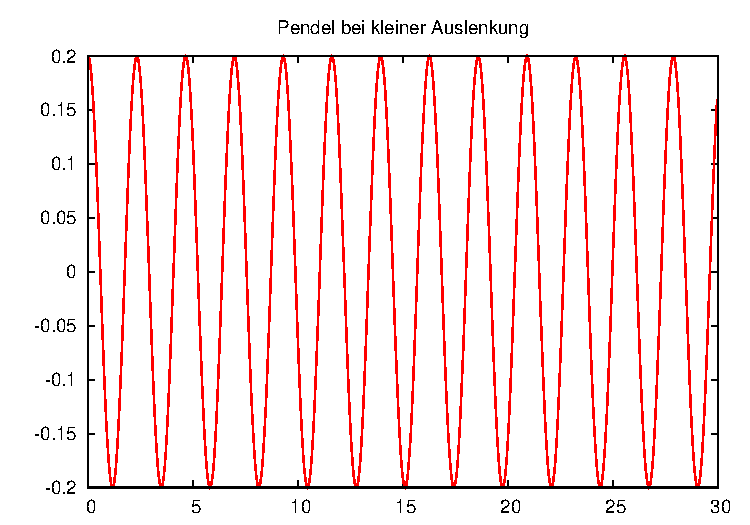
\includegraphics[width=0.4\textwidth]{./pendel}
\end{center}
}
\end{frame}

\note{Demonstration: Visualisierung mit Gnuplot.}

\begin{frame}[fragile]
\frametitle{Aufgabe 3}
\begin{enumerate}
\item Gebt eine Wertetabelle für  f(x) = $x^2$ im Bereich [-50 ,50] aus.
\item Orientiert euch dabei an pendel.cc für das Format der Ausgabe.
\item Plottet die Funktion mit Gnuplot. 
\end{enumerate}
\end{frame}

\mode*

\chapter{Funktionen}
\mode<all>


\begin{frame}[fragile]
\frametitle{Numerische Lösung des Pendels}
\begin{itemize}
\item Volles Modell für das Pendel aus der Einführung:
  \begin{gather*}
    \frac{d^2\phi(t)}{d t^2} = - \frac{g}{l} \sin(\phi(t)) \qquad \forall t>0,\\
    \phi(0) = \phi_0, \qquad \frac{d \phi}{d t}(0) = u_0.
  \end{gather*}
\item Umschreiben in System erster Ordnung:
  \begin{align*}
    \frac{d\phi(t)}{d t} &= u(t), & \frac{d^2\phi(t)}{d t^2} &=
    \frac{d u(t)}{d t} = - \frac{g}{l} \sin(\phi(t)).
  \end{align*}
\item Eulerverfahren für $\phi^n = \phi(n\Delta t)$, $u^n = u(n\Delta t)$:
  \begin{align*}
    \phi^{n+1} &= \phi^n + \Delta t \, u^n & \phi^0 &= \phi_0\\
    u^{n+1} &= u^n -\Delta t \, (g/l) \, \sin(\phi^n) & u^0 &= u_0
  \end{align*}
\end{itemize}
\end{frame}

\begin{frame}[fragile]
\frametitle{Pendel (expliziter Euler)}
\lstinputlisting[basicstyle=\ttfamily\scriptsize,numbers=left,
numberstyle=\tiny, numbersep=5pt]{../examples/progkurs/pendelnumerisch.cc}
\end{frame}

\subsection{Funktionen}

\begin{frame}[fragile]
\frametitle{Funktionsaufruf und Funktionsdefinition}
\begin{itemize}
\item In der Mathematik gibt es das Konzept der \textsl{Funktion}.
\item In C++ auch.
\item Sei $f : \mathbb{R} \to \mathbb{R}$, z.B. $f(x) = x^2$.
\item Wir unterscheiden den \textsl{Funktionsaufruf}
{\scriptsize\begin{lstlisting}{}
double x,y;
y = f(x);
\end{lstlisting}}
\item und die \textsl{Funktionsdefinition}. Diese sieht so aus:

\medskip
\textsl{Ergebnistyp} \textsl{Funktionsname} \lstinline{(} \textsl{Argumente} \lstinline{)}

\lstinline!{! \textsl{Funktionsrumpf} \lstinline!}!

\medskip
\item Beispiel:
{\scriptsize\begin{lstlisting}{}
double f (double x)
{
  return x*x;
}
\end{lstlisting}}
\end{itemize}
\end{frame}

\begin{frame}[fragile]
\frametitle{Komplettbeispiel zur Funktion}
\lstinputlisting[basicstyle=\ttfamily\scriptsize,numbers=left,
numberstyle=\tiny, numbersep=5pt]{../examples/progkurs/funktion.cc}
\begin{itemize}
\item Funktionsdefinition muss vor Funktionsaufruf stehen.
\item Formales Argument in der Funktionsdefinition entspricht einer Variablendefinition.
\item Beim Funktionsaufruf wird das Argument (hier) \textsl{kopiert}.
\item \lstinline{main} ist auch nur eine Funktion.
\end{itemize}
\end{frame}

\begin{frame}[fragile]
\frametitle{Weiteres zum Verständnis der Funktion}
\begin{itemize}
\item Der Name des formalen Arguments in der Funktionsdefinition
  ändert nichts an der Semantik der Funktion (Sofern es überall
  geändert wird):

{\scriptsize\begin{lstlisting}{}
double f (double y)
{
  return y*y;
}
\end{lstlisting}}

\item Das Argument wird hier kopiert, d.h.:
{\scriptsize\begin{lstlisting}{}
double f (double y)
{
  y = 3*y*y;
  return y;
}

int main ()
{
  double x(3.0),y;
  y = f(x); // ändert nichts an x !
}
\end{lstlisting}}
\end{itemize}
\end{frame}

\begin{frame}[fragile]
\frametitle{Weiteres zum Verständnis der Funktion}
\begin{itemize}
\item Argumentliste kann leer sein (wie in der Funktion
  \lstinline{main}):
{\scriptsize\begin{lstlisting}{}
double pi ()
{
  return 3.14;
}

y = pi(); // Klammern sind erforderlich!
\end{lstlisting}}

\item Der Rückgabetyp \lstinline{void} bedeutet \glqq{}keine
  Rückgabe\grqq{}

{\scriptsize\begin{lstlisting}{}
void hello ()
{
  std::cout << "hello" << std::endl;
}

hello();
\end{lstlisting}}
\item Mehrere Argument werden durch Kommata getrennt:

{\scriptsize\begin{lstlisting}{}
double g (int i, double x)
{
  return i*x;
}
std::cout << g(2,3.14) << std::endl;
\end{lstlisting}}
\end{itemize}
\end{frame}

\begin{frame}[fragile]
\frametitle{Pendelsimulation als Funktion}
\lstinputlisting[basicstyle=\ttfamily\scriptsize,numbers=left,
numberstyle=\tiny, numbersep=5pt]{../examples/progkurs/pendelmitfunktion.cc}
\end{frame}

\begin{frame}[fragile]
\frametitle{Aufgabe 4}
\begin{enumerate}
\item Schreibt eine Funktion, die die Fakultät einer (natürlichen) Zahl berechnet und ausgibt.
\item Plottet die Funktion mit Gnuplot im Bereich [1,10]. 
\end{enumerate}
\end{frame}

\begin{frame}[fragile]
\frametitle{Funktionsschablonen}
\begin{itemize}
\item Oft macht eine Funktion mit Argumenten verschiedenen Typs einen Sinn.
\item \lstinline!double f (double x) {return x*x;}! macht auch mit
  \lstinline{float}, \lstinline{int} oder \lstinline{mpf_class} Sinn.
\item Man könnte die Funktion für jeden Typ definieren. Das ist
  natürlich sehr umständlich. (Es darf mehrere Funktionen gleichen
  Namens geben, sog. \textsl{overloading}).
\item In C++ gibt es mit Funktionsschablonen (engl.: \textsl{function
  templates}) eine Möglichkeit den Typ variabel zu lassen:
{\scriptsize\begin{lstlisting}{}
template<typename T>
T f (T y)
{
  return y*y;
}
\end{lstlisting}}
\item \lstinline{T} steht hier für einen beliebigen Typ.
\end{itemize}
\end{frame}

\begin{frame}[fragile,allowframebreaks]
\frametitle{Pendelsimulation mit Templates}
\lstinputlisting[basicstyle=\ttfamily\scriptsize,numbers=left,
numberstyle=\tiny, numbersep=5pt]{../examples/progkurs/pendelmitfunktionstemplate.cc}
\end{frame}


\begin{frame}[fragile]
\frametitle{Headerdateien}
\begin{itemize}
\item Das tolle an Funktionen ist, dass man sie wiederverwenden kann.
\item Es gibt ganze Sammlungen an Funktionen, sogenannte Funktionsbibliotheken
\item Werden in separaten Headerdateien gespeichert. (Dateiendung .h,.hh, o."a.)
\item Um Funktionen (und anderes) aus einer Headerdatei zu verwenden:
\item \#include "Dateiname"
\item Es gibt eine Standardbibliothek von Headerdateien (z.b. cmath,string,iostream)

\end{itemize}
\end{frame}


\begin{frame}[fragile]
\frametitle{Headerdateien}
{\scriptsize\begin{lstlisting}{}
#include <iostream> // Standardbibliothek (Name in <>)
#include <cmath>
#include "hdnum.hh" // Eigene Headerdatei (Dateiname in " \ ")

int main()
{
	float zahl = 5.0;
	zahl = sqrt(zahl); //sqrt aus cmath 
	std::cout << zahl << std::endl; 
	// std::cout, std::endl aus iostream
	hdnum::vector(2,1.0); // Aus hdnum.hh
}
\end{lstlisting}}
\end{frame}

\begin{frame}[fragile]
\frametitle{Headerdateien}
\begin{itemize}
\item Nur \#include in die Datei zu schreiben reicht nicht!
\item Beim kompilieren muss noch der Ort der Headerdatei angegeben werden
\item bei dem kompilierbefehl -I<Verzeichnis> einfügen
\item z.b. g++ -o hallohdnum -I../../ hallohdnum.cc
\item ../../ bedeutet Oberverzeichnis des Oberverzeichnisses (2x ../)

\end{itemize}
\end{frame}


\begin{frame}[fragile]
\frametitle{Aufgabe 5}
\begin{enumerate}
\item Erstellt eine Headerdatei für eure Fakultätsfunktion aus Aufgabe 3. (z.b. fakultaet.hh)
\item Schreibt eure Funktionsdefinition in die Headerdatei, und kommentiert sie in der Hauptdatei aus.
\item Bindet eure headerdatei mit \#include ein und führt eure Funktion in der Datei aus.
\end{enumerate}
\end{frame}
\mode*

\chapter{HDNum}
\mode<all>

\begin{frame}[fragile]
\frametitle{Klassen}
\begin{itemize}
\item Sehr grobe Darstellung von Klassen für die Praktische Verwendung.
\item Klassen erlauben einem C++ Programmierer eigene Datentypen zu definieren.
\item Es gibt unter anderem Klassenvariablen und Klassenmethoden.
\item Klassenvariablen sind die Variablen aus denen der neue Datentyp zusammengesetzt ist.
\item Können elementare Datentypen wie int sein oder aber auch andere Klassen.
\item Klassenmethoden sind Funktionen mit denen Klassenvariablen manipuliert werden können.
\end{itemize}
\end{frame}


\begin{frame}[fragile,allowframebreaks]
\frametitle{Klassen}
\lstinputlisting[basicstyle=\ttfamily\scriptsize,numbers=left,
numberstyle=\tiny, numbersep=5pt]{../examples/progkurs/classes.cc}
\end{frame}



\begin{frame}[fragile]
\frametitle{Klassen III}
\begin{itemize}
\item Klassenvariablen können grundsätzlich nur durch Klassenmethoden modifiziert oder gelesen werden!
\item Ausnahme: Variablen die als "public" deklariert wurden.
\item Verschiedene Variablen einer Klasse (wie eben V und W) teilen sich ihre Untervariablen nicht.
\item Zugriff auf Klassenelemente erfolgt über den . Operator: Also wie eben V.getNorm(), V.x, W.x
\end{itemize}
\end{frame}

\begin{frame}[fragile]
\frametitle{Klassenbibliotheken}
\begin{itemize}
\item Klassen muss man (zum Glück) oft nicht selbst programmieren.
\item Es gibt bereits fertige Klassenbibliotheken.
\item Im folgenden beschäftigen wir uns mit der HDNum-Bibiliothek für den Numerik-Kurs
\end{itemize}
\end{frame}

\begin{frame}[fragile]
\frametitle{HDNUM}
\begin{itemize}
\item C++ kennt keine Matrizen, Vektoren, Polynome, \ldots
\item Wir haben C++ erweitert um die \textbf{Heidelberg Educational
  Numerics Library}, kurz \textbf{HDNum}.
\item Alle in der Vorlesung behandelten Beispiele sind dort
  enthalten.
\item Dieser Programmierkurs ist auch Teil von HDNUM
\end{itemize}
\end{frame}

\begin{frame}[fragile]
\frametitle{HDNUM}
\begin{itemize}
\item HDNum realisiert Vektoren, Matrizen usw. als Klassen-Templates
\item Klassen-Templates analog zu Funktions-Templates
\item d.h. Vektoren, Matrizen mit Elementen verschiedener Datentypen
\item Klassenmethoden für Lineare Algebra, z.b. Matrizenmultiplikation, Skalarprodukte
\item Einbinden über \#include "hdnum.hh"
\item + Angabe des Verzeichnisses der Datei hdnum.hh über -I<Verzeichnis> beim kompilieren
\item Detaillierte Anleitung im repository unter hdnum/tutorial
\end{itemize}
\end{frame}

\begin{frame}[fragile]
\frametitle{HDNUM Vektoren}
\lstinputlisting[basicstyle=\ttfamily\scriptsize,numbers=left,
numberstyle=\tiny, numbersep=5pt]{../examples/progkurs/vektoren.cc}
\end{frame}

\begin{frame}[fragile]
\frametitle{HDNUM Matrizen}
\lstinputlisting[basicstyle=\ttfamily\scriptsize,numbers=left,
numberstyle=\tiny, numbersep=5pt]{../examples/progkurs/matrizen.cc}
\end{frame}

\begin{frame}[fragile]
\frametitle{HDNUM Ausgabe}
\lstinputlisting[basicstyle=\ttfamily\scriptsize,numbers=left,
numberstyle=\tiny, numbersep=5pt]{../examples/progkurs/ausgabe.cc}
\end{frame}


\begin{frame}[fragile]
\frametitle{Beispiel: Gram-Schmidt-Orthogonalisierung mit HDNUM}
\begin{itemize}
\item Gegeben: n (linear unabhängige) Vektoren
\item Gesucht: n orthogonale Vektoren, die den selben Unterraum aufspannen
\item Projektionen der anderen Vektoren werden raussubtrahiert
\item Entsprechend der Formel:


\end{itemize}
\large
\centering
\vspace{0.5cm}
\hspace{2cm}
$ w_{j}=v_{j}-\sum_{i=1}^{j-1} \frac{\left\langle w_{i}, v_{j}\right\rangle}{\left\langle w_{i}, w_{i}\right\rangle} w_{i}$
\end{frame}


\begin{frame}[fragile,allowframebreaks]
\frametitle{Gram-Schmidt Orthogonalisierung}
\lstinputlisting[basicstyle=\ttfamily\scriptsize,numbers=left,
numberstyle=\tiny, numbersep=5pt]{../examples/progkurs/gs.cc}
\end{frame}


\begin{frame}[fragile]
\frametitle{Debugging}
\begin{itemize}
\item Was mache ich wenn mein Programm nicht läuft?
\item Grundsätzliches:
\begin{enumerate}
\item Fehlermeldung lesen!
\item Fehlermeldung bei google eingeben (Copy-Paste) falls unklar.
\item Falls ihr gar nicht weiter kommt: Kommilitonen/Tutoren um Hilfe bitten.
\end{enumerate}
\end{itemize}
\end{frame}

\begin{frame}[fragile]
\frametitle{Debugging II}
\begin{itemize}
\item Was mache ich wenn mein Programm läuft, aber nicht das macht was ich erwarte?
\begin{enumerate}
\item Geht das Programm nochmal Zeile für Zeile durch.
\item Schaut euch den Wert eurer Variablen mit std::cout an.
\item Insbesondere Variablen in If-Statements oder Schleifen.
\item Falls möglich, Ergebnis plotten. (grundsätzlich sinnvoll)
\item Falls ihr gar nicht weiter kommt: Kommilitonen/Tutoren um Hilfe bitten.
\end{enumerate}
\end{itemize}
\end{frame}

\begin{frame}[fragile]
\frametitle{Debugging III}
\begin{itemize}
\item Typische Fehler
\begin{enumerate}
\item Semikolon vergessen
\item Klammer vergessen
\item Gro\ss- und Kleinschreibung
\item Sonstige Tippfehler
\item Variable nicht deklariert/initialisiert
\item Falscher Datentyp in Funktion eingesetzt
\item und vieles mehr...
\end{enumerate}
\end{itemize}
\end{frame}


\mode*



%%%%%%%%%%%%%%%%%%%%%%%%%%%%%%%%%%%%%%%%%%%%%%%%%%%%%%%%%%%%%%%
%%%%%%%%%%%%%%%%%%%%%%%%%%%%%%%%%%%%%%%%%%%%%%%%%%%%%%%%%%%%%%%


% die weiterführende Literatur wollen wir in der Präsentation nie
% zeigen
%\mode<presentation> {
%\begin{frame}<presentation>[allowframebreaks,allowdisplaybreaks]
%  \frametitle{Literatur}
%  \nocite{StoerI}
%  \nocite{Rannacher0}
%  \bibliographystyle{geralpha}
%  \bibliography{lit}
%\end{frame}
%}
%
\end{document}
}
\mode<all>{\section{Vektoren und Matrizen}

\mode<presentation>{
  \begin{frame}<presentation> \frametitle{Inhalt}
    \tableofcontents[currentsection,sectionstyle=show/hide,subsectionstyle=show/show/hide]
  \end{frame}
}

HDNUM stellt Matrix und Vektorklassen zur Verfügung.
\subsection{Vektoren}

\begin{frame}[fragile]
\frametitle{\lstinline{hdnum::Vector<T>}}
\begin{itemize}
\item \lstinline{hdnum::Vector<T>} ist ein Klassen-Template.
\item Es macht aus einem beliebigen (Zahl-)Datentypen \lstinline{T}
  einen Vektor.
\item Auch komplexe und hochgenaue Zahlen sind möglich.
\item Vektoren verhalten sich so wie man es aus der Mathematik kennt:
\begin{itemize}
\item Bestehen aus $n$ Komponenten.
\item Diese sind von $0$ bis $n-1$ (!) durchnummeriert.
\item Addition und Multiplikation mit Skalar.
\item Skalarprodukt und Norm (noch nicht implementiert).
\item Matrix-Vektor-Multiplikation
\end{itemize}
\item Die folgenden Beispiele findet man in \lstinline{vektoren.cc}
\end{itemize}
\end{frame}

\begin{frame}[fragile]
\frametitle{Konstruktion und Zugriff}
\begin{itemize}
\item Konstruktion mit und ohne Initialisierung\\
{\footnotesize{\begin{lstlisting}{}
hdnum::Vector<float> x(10);        // Vektor mit 10 Elementen
hdnum::Vector<double> y(10,3.14);  // 10 Elemente initialisiert
hdnum::Vector<float> a;            // ein leerer Vektor
\end{lstlisting}}}
\item Speziellere Vektoren\\
{\footnotesize{\begin{lstlisting}{}
hdnum::Vector<std::complex<double> >
  cx(7,std::complex<double>(1.0,3.0));
mpf_set_default_prec(1024); // Setze Genauigkeit für mpf\_class
hdnum::Vector<mpf_class> mx(7,mpf_class("4.44"));
\end{lstlisting}}}
\item Zugriff auf Element\\
{\footnotesize{\begin{lstlisting}{}
for (std::size_t i=0; i<x.size(); i=i+1)
  x[i] = i;                 // Zugriff auf Elemente
\end{lstlisting}}}
\item Vektorobjekt wird am Ende des umgebenden Blockes gelöscht.
\end{itemize}
\end{frame}

\begin{frame}[fragile]
\frametitle{Kopie und Zuweisung}
\begin{itemize}
\item Copy-Konstruktor: Erstellen eines Vektors als Kopie eines anderen
{\footnotesize{\begin{lstlisting}{}
hdnum::Vector<float> z(x); // z ist Kopie von x
\end{lstlisting}}}
\item Zuweisung nach Initialisierung, beide Vektoren
müssen die gleiche Größe haben!
{\footnotesize{\begin{lstlisting}{}
b = z;              // b kopiert die Daten aus z
a = 5.4;            // Zuweisung an alle Elemente
hdnum::Vector<double> w;   // leerer Vektor
w.resize(x.size()); // make correct size
w = x;              // copy elements
\end{lstlisting}}}
\item Ausschnitte von Vektoren\\
{\footnotesize{\begin{lstlisting}{}
hdnum::Vector<float> w(x.sub(7,3));// w ist Kopie von x[7],...,x[9]
z = x.sub(3,4);             // z ist Kopie von x[3],...,x[6]
\end{lstlisting}}}
\end{itemize}
\end{frame}

\begin{frame}[fragile]
\frametitle{Rechnen und Ausgabe}
\begin{itemize}
\item Vektorraumoperationen und Skalarprodukt\\
{\footnotesize{\begin{lstlisting}{}
w += z;            // w = w+z
w -= z;            // w = w-z
w *= 1.23;         // skalare Multiplikation
w /= 1.23;         // skalare Division
w.update(1.23,z);  // w = w + a*z
float s;
s = w*z;           // Skalarprodukt
\end{lstlisting}}}
\item Ausgabe auf die Konsole\\
{\footnotesize{\begin{lstlisting}{}
std::cout << w << std::endl;// schöne Ausgabe
w.iwidth(2);                // Stellen in Indexausgabe
w.width(20);                // Anzahl Stellen gesamt
w.precision(16);            // Anzahl Nachkommastellen
std::cout << w << std::endl;// nun mit mehr Stellen
std::cout <<cx << std::endl;// geht auch für complex
std::cout <<mx << std::endl;// geht auch für mpf\_class
\end{lstlisting}}}
\end{itemize}
\end{frame}

\begin{frame}[fragile]
\frametitle{Beispielausgabe}
{\footnotesize{\begin{lstlisting}{}
[   0]    1.204200e+01
[   1]    1.204200e+01
[   2]    1.204200e+01
[   3]    1.204200e+01

[ 0] 1.2042000770568848e+01
[ 1] 1.2042000770568848e+01
[ 2] 1.2042000770568848e+01
[ 3] 1.2042000770568848e+01
\end{lstlisting}}}
\end{frame}

\begin{frame}[fragile]
\frametitle{Hilfsfunktionen}
{\footnotesize{\begin{lstlisting}{}
zero(w);                    // das selbe wie w=0.0
fill(w,(float)1.0);         // das selbe wie w=1.0
fill(w,(float)0.0,(float)0.1); // w[0]=0, w[1]=0.1, w[2]=0.2, ...
unitvector(w,2);            // kartesischer Einheitsvektor
gnuplot("test.dat",w);      // gnuplot Ausgabe: i w[i]
gnuplot("test2.dat",w,z);   // gnuplot Ausgabe: w[i] z[i]
\end{lstlisting}}}
\end{frame}

\begin{frame}[fragile]
\frametitle{Funktionen}
\begin{itemize}
\item Beispiel: Summe aller Komponenten\\
{\footnotesize{\begin{lstlisting}{}
double sum (hdnum::Vector<double> x) {
  double s(0.0);
  for (std::size_t i=0; i<x.size(); i=i+1)
    s = s + x[i];
  return s;
}
\end{lstlisting}}}
\item Mit \textbf{Funktionentemplate}:\\
{\footnotesize{\begin{lstlisting}{}
template<class T>
T sum (hdnum::Vector<T> x) {
  T s(0.0);
  for (std::size_t i=0; i<x.size(); i=i+1)
    s = s + x[i];
  return s;
}
\end{lstlisting}}}
\item \textbf{Vorsicht}: Call-by-value erzeugt \textbf{keine} Kopie!
\end{itemize}
\end{frame}

\subsection{Matrizen}

\begin{frame}[fragile]
\frametitle{\lstinline{hdnum::DenseMatrix<T>}}
\begin{itemize}
\item \lstinline{hdnum::DenseMatrix<T>} ist ein Klassen-Template.
\item Es macht aus einem beliebigen (Zahl-)Datentypen \lstinline{T}
  eine Matrix.
\item Auch komplexe und hochgenaue Zahlen sind möglich.
\item Matrizen verhalten sich so wie man es aus der Mathematik kennt:
\begin{itemize}
\item Bestehen aus $m\times n$ Komponenten.
\item Diese sind von $0$ bis $m-1$ bzw. $n-1$ (!) durchnummeriert.
\item $m\times n$-Matrizen bilden einen Vektorraum.
\item Matrix-Vektor und Matrizenmultiplikation.
\end{itemize}
\item Die folgenden Beispiele findet man in \lstinline{matrizen.cc}
\end{itemize}
\end{frame}

\begin{frame}[fragile]
\frametitle{Konstruktion und Zugriff}
\begin{itemize}
\item Konstruktion mit und ohne Initialisierung\\
{\footnotesize{\begin{lstlisting}{}
hdnum::DenseMatrix<float> B(10,10);     // 10x10 Matrix uninitialisiert
hdnum::DenseMatrix<float> C(10,10,0.0); // 10x10 Matrix initialisiert
\end{lstlisting}}}
\item Zugriff auf Elemente\\
{\footnotesize{\begin{lstlisting}{}
for (int i=0; i<B.rowsize(); ++i)
  for (int j=0; j<B.colsize(); ++j)
    B[i][j] = 0.0;          // jetzt ist B initialisiert
\end{lstlisting}}}
\item Matrixobjekt wird am Ende des umgebenden Blockes gelöscht.
\end{itemize}
\end{frame}

\begin{frame}[fragile]
\frametitle{Kopie und Zuweisung}
\begin{itemize}
\item Copy-Konstruktor: Erstellen einer Matrix als Kopie einer anderen
{\footnotesize{\begin{lstlisting}{}
hdnum::DenseMatrix<float> D(B); // D Kopie von B
\end{lstlisting}}}
\item Zuweisung nach Initialisierung, beide Matrizen müssen gleiche Größe haben:
{\footnotesize{\begin{lstlisting}{}
hdnum::DenseMatrix<float> A(B.rowsize(),B.colsize()); // make correct size
A = B;                    // copy elements
\end{lstlisting}}}
\item Ausschnitte von Matrizen (Untermatrizen)\\
{\footnotesize{\begin{lstlisting}{}
hdnum::DenseMatrix<float> F(A.sub(1,2,3,4));// 3x4 Mat ab (1,2)
\end{lstlisting}}}
\end{itemize}
\end{frame}

\begin{frame}[fragile]
\frametitle{Rechnen mit Matrizen}
\begin{itemize}
\item Vektorraumoperationen\\
{\footnotesize{\begin{lstlisting}{}
A += B;           // A = A+B
A -= B;           // A = A-B
A *= 1.23;        // Multiplikation mit Skalar
A /= 1.23;        // Division durch Skalar
A.update(1.23,B); // A = A + s*B
\end{lstlisting}}}
\item Matrix-Vektor und Matrizenmultiplikation\\
{\footnotesize{\begin{lstlisting}{}
hdnum::Vector<float> x(10,1.0); // make two vectors
hdnum::Vector<float> y(10,2.0);
A.mv(y,x);               // y = A*x
A.umv(y,x);              // y = y + A*x
A.umv(y,(float)-1.0,x);  // y = y + s*A*x
C.mm(A,B);               // C = A*B
C.umm(A,B);              // C = C + A*B
\end{lstlisting}}}
\end{itemize}
\end{frame}

\begin{frame}[fragile]
\frametitle{Ausgabe und Hilfsfunktionen}
\begin{itemize}
\item Ausgabe von Matrizen\\
{\footnotesize{\begin{lstlisting}{}
std::cout << A.sub(0,0,3,3) << std::endl;// schöne Ausgabe
A.iwidth(2);                // Stellen in Indexausgabe
A.width(10);                // Anzahl Stellen gesamt
A.precision(4);             // Anzahl Nachkommastellen
std::cout << A << std::endl;// nun mit mehr Stellen
\end{lstlisting}}}
\item einige Hilfsfunktionen
{\footnotesize{\begin{lstlisting}{}
identity(A);
spd(A);
fill(x,(float)1,(float)1);
vandermonde(A,x);
\end{lstlisting}}}
\end{itemize}
\end{frame}

\begin{frame}[fragile]
\frametitle{Beispielausgabe}
{\footnotesize{\begin{lstlisting}{}
               0           1           2           3
  0   4.0000e+00 -1.0000e+00 -2.5000e-01 -1.1111e-01
  1  -1.0000e+00  4.0000e+00 -1.0000e+00 -2.5000e-01
  2  -2.5000e-01 -1.0000e+00  4.0000e+00 -1.0000e+00
  3  -1.1111e-01 -2.5000e-01 -1.0000e+00  4.0000e+00
\end{lstlisting}}}
\end{frame}

\begin{frame}[fragile]
\frametitle{Funktion mit Matrixargument}
Beispiel einer Funktion, die eine Matrix $A$ und einen Vektor $b$
initialisiert.

{\footnotesize{\begin{lstlisting}{}
template<class T>
void initialize (hdnum::DenseMatrix<T> A, hdnum::Vector<T> b)
{
  if (A.rowsize()!=A.colsize() || A.rowsize()==0)
    HDNUM_ERROR("need square and nonempty matrix");
  if (A.rowsize()!=b.size())
    HDNUM_ERROR("b must have same size as A");
  for (int i=0; i<A.rowsize(); ++i)
    {
      b[i] = 1.0;
      for (int j=0; j<A.colsize(); ++j)
        if (j<=i) A[i][j]=1.0; else A[i][j]=0.0;
    }
}
\end{lstlisting}}}
\end{frame}
}
\mode<all>{\section{Gewöhnliche Differentialgleichungen}

\mode<presentation>{
  \begin{frame}<presentation> \frametitle{Inhalt}
    \tableofcontents[currentsection,sectionstyle=show/hide,subsectionstyle=show/show/hide]
  \end{frame}
}

\subsection{Differentialgleichungsmodelle und Löser}

\begin{frame}[fragile]
\frametitle{Gewöhnliche Differentialgleichungen in HDNUM}
\begin{itemize}
\item Erlaube Lösung beliebiger Modelle mit beliebigen Lösern.
\item Erlaube variable Typen für Zeit und Zustand.
\item Trenne folgende Komponenten:
\begin{itemize}
\item Differentialgleichungsmodell (inklusive Anfangsbedingung),
\item Lösungsverfahren,
\item Steuerung und Zeitschleife.
\end{itemize}
\end{itemize}
\end{frame}

\begin{frame}[fragile]
\frametitle{Differentialgleichungsmodell}
Ein Differentialgleichungsmodell ist gegeben durch
\begin{itemize}
\item Typen für Zeit und Zustandskomponenten variabel.
\item Größe des Systems $d$.
\item Anfangszustand $(t_0,u_0)$.
\item Funktion $f(t,x) : \mathbb{R}\times\mathbb{R}^d \to \mathbb{R}^d$.
\item Optional die Jacobimatrix $f_x(t,x)$ (wird für implizite Verfahren benötigt).
\item Für Zustand und Jacobimatrix verwenden wir Vektor- und Matrixklassen aus HDNUM.
\end{itemize}
Als nächstes ein Beispiel für das Modellproblem
\begin{equation*}
u'(t) = \lambda u(t), \quad t\geq t_0, \quad u(t_0)=u_0, \quad \lambda\in\mathbb{R}, \mathbb{C}.
\end{equation*}
\end{frame}

\begin{frame}[fragile,allowframebreaks,allowdisplaybreaks]
\frametitle{Modellproblem}
\framesubtitle{(Datei \texttt{examples/num1/modelproblem.hh})}
\lstinputlisting[basicstyle=\tiny,numbers=left,
numberstyle=\tiny, numbersep=2pt]{../examples/num1/modelproblem.hh}
\end{frame}

\begin{frame}[fragile]
\frametitle{Differentialgleichungslöser}
\begin{itemize}
\item Differentialgleichungsmodell ist ein Template-Parameter.
\item Typen für Zeit und Zustand werden aus Differentialgleichungsmodell genommen.
\item Kapselt aktuellen Zustand und aktuelle Zeit (und evtl. weitere Zustände).
\item Methode \lstinline{step} führt einen Schritt des Verfahrens durch.
\end{itemize}
Als nächstes ein Beispiel für den expliziten Euler.
\end{frame}

\begin{frame}[fragile,allowframebreaks,allowdisplaybreaks]
\frametitle{Expliziter Euler}
\framesubtitle{(Datei \texttt{examples/num1/expliciteuler.hh})}
\lstinputlisting[basicstyle=\tiny,numbers=left,
numberstyle=\tiny, numbersep=2pt]{../examples/num1/expliciteuler.hh}
\end{frame}

\begin{frame}[fragile]
\frametitle{Lösung und Ergebnisausgabe}
Die Lösung eines Differentialgleichungsmodells besteht nun aus
\begin{itemize}
\item Instantieren der entsprechenden Objekte für Modell und Löser.
\item Zeitschrittschleife bis zur gewünschten Endzeit.
\item Speicherung und Ausgabe der Ergebnisse in einem \lstinline{hdnum::Vector}.
\item Visualisierung der Ergebnisse mit \lstinline{gnuplot}.
\end{itemize}
\end{frame}

\begin{frame}[fragile,allowframebreaks,allowdisplaybreaks]
\frametitle{Hauptprogramm für Modellproblem}
\framesubtitle{(Datei \texttt{examples/num1/modelproblem.cc})}
\lstinputlisting[basicstyle=\tiny,numbers=left,
numberstyle=\tiny, numbersep=2pt]{../examples/num1/modelproblem.cc}
\end{frame}
}

%%%%%%%%%%%%%%%%%%%%%%%%%%%%%%%%%%%%%%%%%%%%%%%%%%%%%%%%%%%%%%%
%%%%%%%%%%%%%%%%%%%%%%%%%%%%%%%%%%%%%%%%%%%%%%%%%%%%%%%%%%%%%%%


% die weiterführende Literatur wollen wir in der Präsentation nie
% zeigen
\mode<presentation> {
\begin{frame}<presentation>[allowframebreaks,allowdisplaybreaks]
  \frametitle{Literatur}
  \nocite{StoerI}
%  \nocite{Deuflhard}
%  \nocite{StoerII}
  \nocite{Rannacher0}
%  \nocite{Schwarz}
%  \nocite{GolubOrtega}
%  \nocite{GolubVanLoan}
%  \nocite{CDE}
%  \nocite{SchabackWendland}
%  \nocite{QuarteroniSaccoSaleri}
  \bibliographystyle{geralpha}
  \bibliography{lit}
\end{frame}
}

% Literatur im Artikel am Schluss
\mode<article> {
  \nocite{StoerI}
  \nocite{Deuflhard}
  \nocite{StoerII}
  \nocite{Rannacher0}
  \nocite{Schwarz}
  \nocite{GolubOrtega}
  \nocite{GolubVanLoan}
  \nocite{CDE}
  \nocite{SchabackWendland}
  \nocite{QuarteroniSaccoSaleri}
  \bibliographystyle{plain}
  \bibliography{lit}
}

\end{document}
